\documentclass[aspectratio=169, table]{beamer}

\usepackage{listings}

\graphicspath{{../../images/}}
%\usepackage[beamertheme=./praditatheme]{Pradita}

\lstdefinestyle{JavaStyle}{
	language=Java,
	basicstyle=\ttfamily\scriptsize,
	keywordstyle=\color{blue},
	commentstyle=\color{gray},
	stringstyle=\color{red},
	breaklines=true,
	showstringspaces=false,
	tabsize=2,
	captionpos=b,
	numbers=left,
	numberstyle=\tiny\color{gray},
	frame=lines,
	backgroundcolor=\color{lightgray!10},
	comment=[l]{//},
	morecomment=[s]{/*}{*/},
	commentstyle=\color{gray}\ttfamily,
	string=[s]{'}{'},
	morestring=[s]{"}{"},
	%	stringstyle=\color{teal}\ttfamily,
	%	showstringspaces=false
}


\usetheme{Pradita}

\title{\Huge Ports and Adapaters\\Architecture\\\vspace{10pt}}
\subtitle{IF231303-Software Architecture}
\author{Alfa Yohannis}
\begin{document}

	\begin{frame}[plain]
		\maketitle
	\end{frame}

	\begin{frame}[fragile]
		\frametitle{Contents}
		
		\begin{columns}[t]
			\column{0.5\textwidth}
			\tableofcontents[sections={1-6}]
			
			\column{0.5\textwidth}
			\tableofcontents[sections={7-12}]
		\end{columns}
	\end{frame}

\section{Introduction}

\section{Introduction}

\begin{frame}[fragile]{Introduction}
	\vspace{20pt}
	In software development, choosing the right architecture is essential for building applications that are:
	\begin{itemize}
		\item \textbf{Flexible} – Able to adapt to evolving business needs.
		\item \textbf{Scalable} – Supporting growth without major redesign.
		\item \textbf{Maintainable} – Easy to update and debug over time.
	\end{itemize}
	A major challenge in software development is managing dependencies between business logic and external technologies such as:
	\begin{itemize}
		\item Databases
		\item APIs
		\item User interfaces
	\end{itemize}
\end{frame}

\begin{frame}[fragile]{Hexagonal Architecture}
	\vspace{20pt}
	Hexagonal Architecture, also known as the \textbf{Ports and Adapters Architecture}, was introduced by \textbf{Alistair Cockburn} in 2005 to:
	\begin{itemize}
		\item \textbf{Decouple} business logic from external technologies.
		\item \textbf{Improve testability} by allowing external dependencies to be replaced with mocks or stubs.
		\item \textbf{Enhance modularity} by enforcing a structured separation between application components.
	\end{itemize}
\end{frame}

\begin{frame}[fragile]{Purpose of This Session}
	\vspace{20pt}
	This session covers the fundamental concepts, principles, and implementation of \textbf{Hexagonal Architecture} in \textbf{Java}. By adopting this approach, developers can create applications that:
	\begin{itemize}
		\item Are \textbf{well-structured} and easy to extend.
		\item Are \textbf{isolated} from changes in external technologies.
		\item \textbf{Facilitate testing} by avoiding direct dependencies on databases or APIs.
	\end{itemize}
\end{frame}

\section{Background}

\begin{frame}[fragile]{The Importance of Software Architecture}
	\vspace{20pt}
	Application architecture defines how different components interact. Traditional architectures, such as \textbf{layered architecture} (\textit{n-tier architecture}), often introduce:
	\begin{itemize}
		\item \textbf{Strong dependencies} between layers.
		\item \textbf{Rigid coupling}, making modifications difficult.
		\item \textbf{Scalability limitations}, due to tightly integrated components.
	\end{itemize}
\end{frame}

\begin{frame}[fragile]{The Evolution Towards Flexible Architectures}
	\vspace{20pt}
	To overcome these limitations, modern architectures focus on flexibility and modularity. \textbf{Hexagonal Architecture} provides several advantages:
	\begin{itemize}
		\item \textbf{Separates} business logic from external technologies like databases, APIs, and UI.
		\item \textbf{Minimizes impact} of technology changes on core application logic.
		\item \textbf{Improves scalability} and maintainability over time.
	\end{itemize}
\end{frame}

\begin{frame}[fragile]{The Ports and Adapters Concept}
	\vspace{20pt}
	Hexagonal Architecture relies on two key principles:
	\begin{itemize}
		\item \textbf{Ports:} Define the interface for external communication.
		\item \textbf{Adapters:} Implement the ports to integrate with specific technologies.
	\end{itemize}
	
	\textbf{Key Benefits:}
	\begin{itemize}
		\item \textbf{Enhances flexibility} by allowing technology-independent business logic.
		\item \textbf{Facilitates unit testing} without external dependencies.
		\item \textbf{Supports modular development} with loosely coupled components.
	\end{itemize}
\end{frame}

\subsection{History of Hexagonal Architecture}

\begin{frame}[fragile]{The Need for Hexagonal Architecture}
	\vspace{20pt}
	\textbf{Origins of Hexagonal Architecture:}
	\begin{itemize}
		\item \textbf{Modular design} that separates concerns.
		\item \textbf{Testability} using mock implementations without external dependencies.
		\item \textbf{Flexibility} to adapt to technology changes without impacting business logic.
	\end{itemize}
	
	\textbf{The Need for a New Approach:}
	\begin{itemize}
		\item Monolithic applications in the early 2000s were tightly coupled to specific frameworks and technologies.
		\item Migration to new architectures was difficult due to these strong dependencies.
		\item Maintenance costs were high because business logic and infrastructure were intertwined.
	\end{itemize}
\end{frame}


\begin{frame}[fragile]{Alistair Cockburn’s Contribution \& Influences}
	\vspace{20pt}
	\textbf{Alistair Cockburn’s Contribution:}
	\begin{itemize}
		\item Introduced the Hexagonal Architecture concept.
		\item Used \textbf{ports} and \textbf{adapters} to isolate business logic from external technologies.
		\item Enabled independent testing from databases, APIs, and other external systems.
		\item Supported seamless integration with evolving technologies without changing core functionality.
	\end{itemize}
	
	\textbf{Influences on Modern Software Development:}
	\begin{itemize}
		\item Inspired \textbf{Clean Architecture} by \textbf{Robert C. Martin} (Uncle Bob).
		\item Aligned with \textbf{Domain-Driven Design (DDD)} by \textbf{Eric Evans}.
		\item Addressed growing demand for flexible, technology-agnostic software architectures.
	\end{itemize}
\end{frame}


\subsection{Motivation for Using Hexagonal Architecture}

\begin{frame}[fragile]{Why Hexagonal Architecture?}
	\vspace{20pt}
	The increasing adoption of Hexagonal Architecture is driven by:
	\begin{itemize}
		\item \textbf{Decoupling business logic from technology dependencies}.
		\item \textbf{Improving unit and integration testing}.
		\item \textbf{Ensuring flexibility in switching technologies}.
		\item \textbf{Supporting modular and scalable software design}.
	\end{itemize}
\end{frame}

\begin{frame}[fragile]{\Large{Decoupling Business Logic and Enhancing Testability}}
	\vspace{20pt}
	\textbf{Decoupling Business Logic:}
	\begin{itemize}
		\item Changes in database technology, framework versions, or external integrations do not impact the core domain logic.
	\end{itemize}
	
	\textbf{Enhancing Testability:}
	\begin{itemize}
		\item Eliminates direct dependencies on external systems.
		\item Allows unit testing without database connections.
		\item Supports integration testing using mock services.
		\item Improves test reliability and execution speed.
	\end{itemize}
\end{frame}

\begin{frame}[fragile]{Technology Flexibility and Scalability}
	\vspace{20pt}
	\textbf{Hexagonal Architecture provides:}
	\begin{itemize}
		\item Easy replacement of databases, message brokers, or UI frameworks.
		\item Minimal code changes when migrating to new infrastructure.
		\item A future-proof software design adaptable to evolving technologies.
		\item Independent feature development and reduced system-wide impact.
		\item Support for distributed and microservices-based architectures.
	\end{itemize}
\end{frame}


\section{Definition, Principles, and Structure of Hexagonal Architecture}

\begin{frame}[fragile]{What is Hexagonal Architecture?}
	\vspace{20pt}
	Hexagonal Architecture, also known as the \textbf{Ports and Adapters Architecture}, is a software architecture pattern designed to:
	\begin{itemize}
		\item \textbf{Separate core business logic} from external technologies like databases, APIs, and user interfaces.
		\item \textbf{Enable technology flexibility} by allowing external dependencies to be swapped without modifying business logic.
		\item \textbf{Improve maintainability} by ensuring a clear boundary between application layers.
	\end{itemize}
\end{frame}

\begin{frame}[fragile]{How It Works}
	\vspace{20pt}
	Hexagonal Architecture ensures that:
	\begin{itemize}
		\item The system interacts with the external world via clearly defined \textbf{ports}.
		\item \textbf{Adapters} implement these ports to facilitate communication with specific technologies.
		\item No direct dependencies exist between business logic and external systems.
	\end{itemize}
\end{frame}

\subsection{Principles of Hexagonal Architecture}

\begin{frame}[fragile]{Core Principles}
	\vspace{20pt}
	Hexagonal Architecture is built upon several key principles:
	\begin{itemize}
		\item \textbf{Separation of Business Logic and External Technologies}  
		The business logic resides in the \textbf{core domain}, while external technologies (databases, services, UI) interact with it only through \textbf{ports and adapters}.
		
		\item \textbf{Interaction via Ports and Adapters}  
		All communication between business logic and the external world happens through:
		\begin{itemize}
			\item \textbf{Ports} – Define the expected interactions.
			\item \textbf{Adapters} – Implement the ports to interact with databases, APIs, or user interfaces.
		\end{itemize}
	\end{itemize}
\end{frame}

\begin{frame}[fragile]{Testing and Flexibility}
	\vspace{20pt}
	Hexagonal Architecture also provides:
	\begin{itemize}
		\item \textbf{Easier Unit Testing}  
		Business logic can be tested independently using mocks or stubs without requiring a real database or external system.
		
		\item \textbf{Technology Agnosticism}  
		Since external technologies are connected via adapters, the system can:
		\begin{itemize}
			\item Replace a database (e.g., switch from MySQL to PostgreSQL) without modifying business logic.
			\item Swap frameworks or messaging systems without affecting the core application.
		\end{itemize}
	\end{itemize}
\end{frame}

\subsection{Structure of Hexagonal Architecture}

\begin{frame}[fragile]{Hexagonal Architecture Structure}
	\vspace{20pt}
	Hexagonal Architecture consists of three main components:
	\begin{itemize}
		\item \textbf{Domain} – The core application logic.
		\item \textbf{Ports} – Interfaces that define communication between the domain and external components.
		\item \textbf{Adapters} – Implementations that connect the system to databases, APIs, and UIs.
	\end{itemize}
\end{frame}

\begin{frame}[fragile]{Hexagonal Architecture}
	\vspace{20pt}
	\begin{figure}[h]
		\centering
		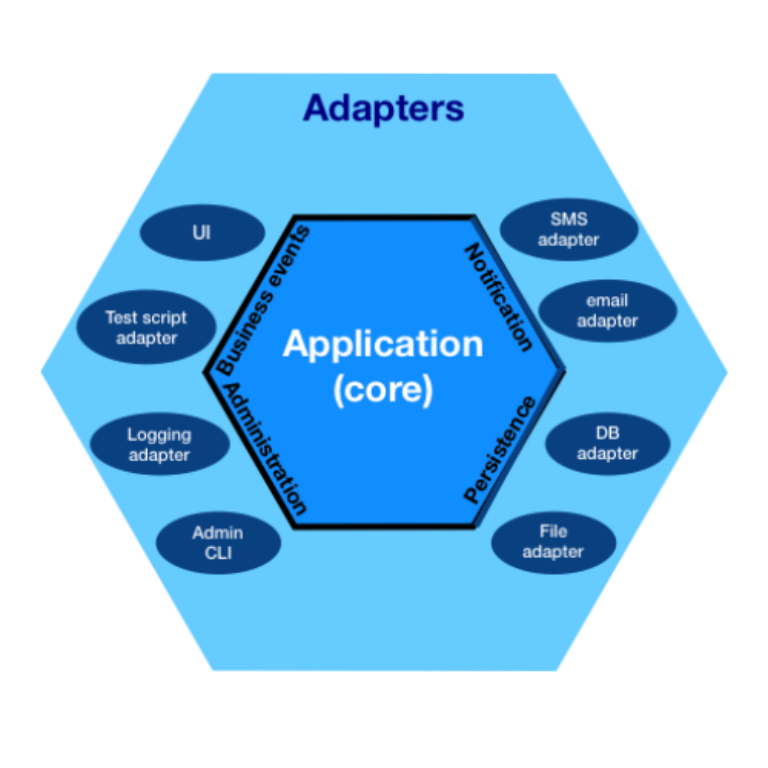
\includegraphics[width=.6\textwidth]{../images/hexagonal_architecture.png}
		\label{fig:hexagonal_architecture}
	\end{figure}
\end{frame}

\begin{frame}[fragile]{Key Components of Hexagonal Architecture}
	\vspace{20pt}
	\textbf{1. Domain}  
	\begin{itemize}
		\item The \textbf{core} of the application that contains all business logic.
		\item Remains independent of any specific technology or framework.
	\end{itemize}
	
	\textbf{2. Ports}  
	\begin{itemize}
		\item Define how external systems interact with the domain.
		\item Ensure the core logic is decoupled from specific technologies.
	\end{itemize}
	
	\textbf{3. Adapters}  
	\begin{itemize}
		\item Serve as bridges between external systems and the domain.
		\item Implement the defined \textbf{ports} to interact with:
		\begin{itemize}
			\item Databases (e.g., MySQL, PostgreSQL).
			\item Messaging systems (e.g., Kafka, RabbitMQ).
			\item Web interfaces (e.g., REST APIs, GraphQL).
		\end{itemize}
	\end{itemize}
\end{frame}


\section{Advantages of Hexagonal Architecture}

\begin{frame}[fragile]{Key Benefits of Hexagonal Architecture}
	\vspace{20pt}
	Hexagonal Architecture offers several advantages in software development, particularly in:
	\begin{itemize}
		\item \textbf{Modularity} – Improves code organization.
		\item \textbf{Ease of testing} – Simplifies unit and integration tests.
		\item \textbf{Flexibility} – Supports changes in external technologies.
		\item \textbf{Maintainability} – Facilitates long-term software evolution.
	\end{itemize}
\end{frame}

\begin{frame}[fragile]{Separation and Testability}
	\vspace{20pt}
	\textbf{Separation of Business Logic and External Technology:}
	\begin{itemize}
		\item Business logic is centralized in the \textbf{domain} layer.
		\item Interactions with external technologies (databases, APIs, messaging systems) occur only through \textbf{ports} and \textbf{adapters}.
		\item Ensures technology changes do not affect core business logic.
	\end{itemize}
	
	\textbf{Improved Unit and Integration Testing:}
	\begin{itemize}
		\item The domain layer’s independence simplifies testing.
		\item \textbf{Mocks} simulate external dependencies.
		\item \textbf{Stubs} provide predefined test responses.
		\item Results in faster, infrastructure-free testing cycles.
	\end{itemize}
\end{frame}


\begin{frame}[fragile]{Flexible and Modular Architecture}
	\vspace{20pt}
	\textbf{Flexibility in Technology Choices:}
	\begin{itemize}
		\item External technologies are connected via \textbf{adapters}, allowing easy replacement.
		\item Examples:  
		\begin{itemize}
			\item Begin with \textbf{MySQL}, then transition to \textbf{MongoDB} without altering business logic.
			\item Migrate from REST APIs to GraphQL with minimal changes.
		\end{itemize}
		\item Reduces the long-term impact of initial technology decisions.
	\end{itemize}
	
	\textbf{Modular and Scalable Structure:}
	\begin{itemize}
		\item The application is divided into:
		\begin{itemize}
			\item \textbf{Domain:} Business rules.
			\item \textbf{Ports:} System interaction contracts.
			\item \textbf{Adapters:} External integration implementations.
		\end{itemize}
		\item Components can be developed and maintained independently.
		\item Enables teams to work in parallel, improving scalability and efficiency.
	\end{itemize}
\end{frame}


\begin{frame}[fragile]{Key Benefits of Hexagonal Architecture}
	\vspace{20pt}
	\textbf{Alignment with Best Practices:}
	\begin{itemize}
		\item \textbf{Separation of Concerns (SoC):} Distinguishes business logic from external dependencies.
		\item \textbf{Dependency Inversion Principle (DIP):} High-level modules rely on abstractions rather than low-level implementations.
		\item \textbf{SOLID Principles:} Encourages maintainable, modular, and extensible codebases.
	\end{itemize}
	
	\textbf{Advantages for Modern Systems:}
	\begin{itemize}
		\item \textbf{Flexibility:} Easily adapts to changing technologies and requirements.
		\item \textbf{Scalability:} Modular components streamline system expansion.
		\item \textbf{Long-term Maintainability:} Ensures a clean separation of concerns, making systems easier to understand and maintain.
	\end{itemize}
\end{frame}


\section{Disadvantages of Hexagonal Architecture}

\begin{frame}[fragile]{Challenges in Hexagonal Architecture}
	\vspace{20pt}
	Despite its many advantages, Hexagonal Architecture also has some drawbacks that should be considered before implementation:
	\begin{itemize}
		\item \textbf{Additional complexity in design}
		\item \textbf{Increased code volume}
		\item \textbf{Steep learning curve}
		\item \textbf{Not always suitable for simple applications}
		\item \textbf{Potential overhead in component communication}
	\end{itemize}
\end{frame}

\begin{frame}[fragile]{Complexity and Code Volume}
	\vspace{20pt}
	\textbf{Increased Design Complexity:}
	\begin{itemize}
		\item Introduces additional layers, including \textbf{ports} and \textbf{adapters}.
		\item Requires detailed architectural planning to keep complexity manageable.
		\item Developers need a strong understanding of Hexagonal Architecture principles to fully leverage its advantages.
	\end{itemize}
	
	\textbf{Higher Code Volume:}
	\begin{itemize}
		\item Additional code results from the strict separation between \textbf{domain}, \textbf{ports}, and \textbf{adapters}.
		\item The initial setup can extend development timelines relative to simpler architectural approaches.
		\item Maintenance efforts increase since multiple components must be updated and tested independently.
	\end{itemize}
\end{frame}


\begin{frame}[fragile]{Challenges and Suitability}
	\vspace{20pt}
	\textbf{Steep Learning Curve:}
	\begin{itemize}
		\item Requires a solid understanding of Hexagonal Architecture concepts, which can take time to master.
		\item Teams may need to invest extra effort in learning best practices before implementation becomes efficient.
		\item Can initially slow down development as developers become proficient with the approach.
	\end{itemize}
	
	\textbf{Not Always Suitable for Simple Applications:}
	\begin{itemize}
		\item For small or straightforward applications, Hexagonal Architecture may introduce unnecessary complexity.
		\item The additional layers and abstractions might not yield sufficient benefits for projects with basic requirements.
		\item In such cases, simpler traditional architectures can often be more practical and cost-effective.
	\end{itemize}
\end{frame}


\begin{frame}[fragile]{Hexagonal Architecture: Overhead and Considerations}
	\vspace{20pt}
	\textbf{Potential Communication Overhead:}
	\begin{itemize}
		\item All domain interactions with external technologies must pass through \textbf{ports} and \textbf{adapters}.
		\item This additional layer can introduce minor performance overhead, especially in high-throughput scenarios.
	\end{itemize}
	
	\textbf{Conclusion:}
	\begin{itemize}
		\item Despite some performance trade-offs, Hexagonal Architecture is well-suited for systems requiring:
		\begin{itemize}
			\item \textbf{Flexibility and scalability.}
			\item \textbf{Strong testability and maintainability.}
			\item \textbf{Long-term technology independence.}
		\end{itemize}
	\end{itemize}
\end{frame}


\section{Java Implementation Example}

\begin{frame}[fragile]{Hexagonal Architecture in Java}
	\vspace{20pt}
	To understand how Hexagonal Architecture can be applied in software development using Java, we present an example with a **customer account management system**.
	
	\textbf{This implementation consists of three main components:}
	\begin{itemize}
		\item \textbf{Domain} – Core business logic, independent of external technologies.
		\item \textbf{Adapters} – Implementation that connects the domain to external systems like databases.
		\item \textbf{Application Services} – Manages interactions between the domain and external clients.
	\end{itemize}
\end{frame}

\begin{frame}[fragile]{Hexagonal Architecture}
	\vspace{20pt}
	\begin{figure}[h]
		\centering
		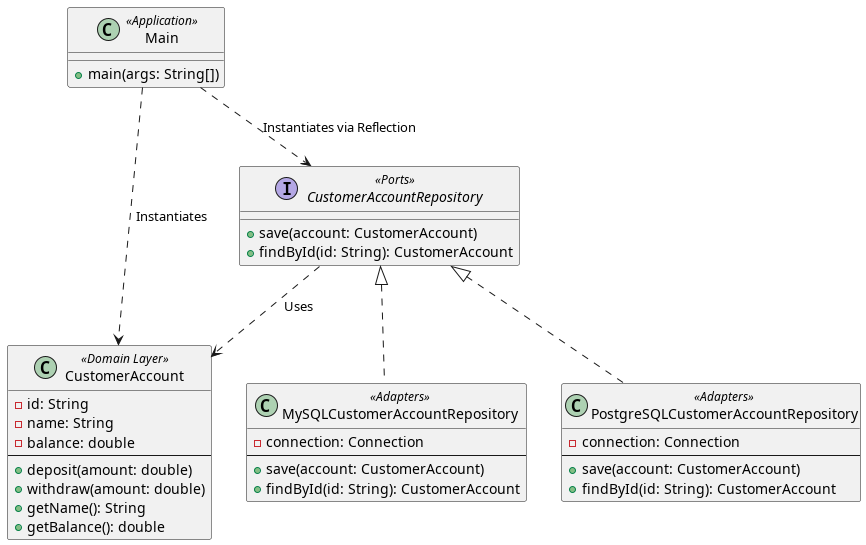
\includegraphics[width=.85\textwidth]{../images/out/hexagonal_component_diagram.png}
		\label{fig:hexagonal_class_diagram}
	\end{figure}
\end{frame}


\section{Domain Definition}
\begin{frame}[fragile]{The Role of the Domain}
	\vspace{20pt}
	The \textbf{Domain} is the core of the system and contains the main business logic. 
	
	\textbf{Key Characteristics:}
	\begin{itemize}
		\item Must be independent of external technologies such as databases, frameworks, or UI.
		\item Ensures business logic remains pure (\textit{pure business logic}).
		\item Can be reused without depending on specific implementations.
	\end{itemize}
	
	\textbf{Use Case: Customer Account Management}
	\begin{itemize}
		\item \textbf{Validating accounts} – Ensures accounts have valid initial balances.
		\item \textbf{Processing balance updates} – Handles deposits and withdrawals.
		\item \textbf{Handling transactions} – Prevents unauthorized withdrawals.
	\end{itemize}
\end{frame}


\begin{frame}[fragile]{Customer Account Entity - Part 1}
	\vspace{20pt}
	\begin{lstlisting}[style=JavaStyle]
		public class CustomerAccount {
			private String id;
			private String name;
			private double balance;
			
			public CustomerAccount(String id, String name, double initialBalance) {
				if (initialBalance < 0) {
					throw new IllegalArgumentException("Initial balance cannot be negative.");
				}
				this.id = id;
				this.name = name;
				this.balance = initialBalance;
			}
			
			public String getId() { return id; }
			public String getName() { return name; }
			public double getBalance() { return balance; }
		}
	\end{lstlisting}
\end{frame}

\begin{frame}[fragile]{Customer Account Entity - Part 2}
	\vspace{20pt}
	\begin{lstlisting}[style=JavaStyle]
		public void deposit(double amount) {
			if (amount <= 0) {
				throw new IllegalArgumentException("Deposit amount must be greater than zero.");
			}
			this.balance += amount;
		}
	\end{lstlisting}
\end{frame}

\begin{frame}[fragile]{Customer Account Entity - Part 3}
	\vspace{20pt}
	\begin{lstlisting}[style=JavaStyle]
		public void withdraw(double amount) {
			if (amount <= 0) {
				throw new IllegalArgumentException("Withdrawal amount must be greater than zero.");
			}
			if (amount > this.balance) {
				throw new IllegalArgumentException("Insufficient balance.");
			}
			this.balance -= amount;
		}
	}
\end{lstlisting}
\end{frame}


\begin{frame}[fragile]{Entity Breakdown: CustomerAccount}
	\vspace{20pt}
	\textbf{The \texttt{CustomerAccount} class represents a customer’s account with:}
	\begin{itemize}
		\item \textbf{\texttt{id}} – Unique identifier for the customer.
		\item \textbf{\texttt{name}} – Customer’s name.
		\item \textbf{\texttt{balance}} – Account balance.
	\end{itemize}
	
	\textbf{Operations within the domain:}
	\begin{itemize}
		\item Constructor ensures that the initial balance is not negative.
		\item \texttt{deposit()} method allows adding funds with a validation check.
		\item \texttt{withdraw()} ensures withdrawals are valid and within available balance.
	\end{itemize}
\end{frame}

\begin{frame}[fragile]{Business Logic in the Domain}
	\vspace{20pt}
	Hexagonal Architecture places business logic in the \textbf{domain} to ensure:
	\begin{itemize}
		\item \textbf{Consistency} – Business rules remain uniform across the application.
		\item \textbf{Testability} – Logic can be tested independently using mocks or stubs.
		\item \textbf{Flexibility} – External system changes do not impact core logic.
	\end{itemize}
	
	\textbf{Benefits of a Clean Domain:}
	\begin{itemize}
		\item \textbf{Scalability} – Business logic can evolve without modifying infrastructure.
		\item \textbf{Technology Independence} – Switching databases, messaging systems, or UI frameworks is simplified.
		\item \textbf{Maintainability} – A modular system allows easier long-term modifications.
	\end{itemize}
\end{frame}


\section{Definition of Ports}

\begin{frame}[fragile]{What is a Port in Hexagonal Architecture?}
	\vspace{20pt}
	In \textbf{Hexagonal Architecture}, a \textbf{port} is an interface that defines how domain components interact with external systems such as:
	\begin{itemize}
		\item Database services
		\item External systems (APIs, messaging queues, etc.)
		\item User interfaces
	\end{itemize}
	\textbf{Purpose:}  
	\begin{itemize}
		\item Acts as a bridge between the domain and external technologies.
		\item Enables communication without creating direct dependencies.
	\end{itemize}
\end{frame}

\begin{frame}[fragile]{The Role of Ports in Hexagonal Architecture}
	\vspace{20pt}
	Ports play a crucial role in maintaining modularity and flexibility:
	\begin{itemize}
		\item \textbf{Separates business logic from external technologies}  
		– The domain does not need to know technical details about how data is stored or how services operate.
		\item \textbf{Defines communication contracts}  
		– Ports specify the interfaces that external technologies (e.g., databases, APIs) must implement.
		\item \textbf{Facilitates unit testing}  
		– Using ports allows testing with \textbf{mocks} or \textbf{stubs}, avoiding reliance on real implementations.
		\item \textbf{Allows technology changes without affecting the domain}  
		– If storage technology changes (e.g., MySQL to MongoDB), only the adapter needs modification, while the business logic remains unchanged.
	\end{itemize}
\end{frame}

\begin{frame}[fragile]{Types of Ports in Hexagonal Architecture}
	\vspace{20pt}
	In Hexagonal Architecture, ports are categorized into two main types:
	\begin{itemize}
		\item \textbf{Inbound Port (Driving Port)}  
		\begin{itemize}
			\item Used to receive external requests and forward them to the domain.
			\item Examples: API services, user interfaces.
		\end{itemize}
		\item \textbf{Outbound Port (Driven Port)}  
		\begin{itemize}
			\item Used by the domain to communicate with external systems such as databases or external services.
			\item The domain calls this port, but its implementation is defined by an adapter.
		\end{itemize}
	\end{itemize}
\end{frame}

\begin{frame}[fragile]{Port Implementation in Java}
	\vspace{20pt}
	In a customer account management system, a \textbf{port} connects the domain with the persistence layer.  
	\textbf{Example: CustomerAccountRepository}
	
	\begin{lstlisting}[style=JavaStyle, caption=CustomerAccountRepository Port]
		public interface CustomerAccountRepository {
			void save(CustomerAccount account);
			CustomerAccount findById(String id);
		}
	\end{lstlisting}
\end{frame}

\begin{frame}[fragile]{Ports in Hexagonal Architecture}
	\vspace{20pt}
	\textbf{Understanding \texttt{CustomerAccountRepository}:}
	\begin{itemize}
		\item Defines a contract for storing and retrieving customer accounts.
		\item \texttt{save(CustomerAccount account)} method saves or updates an account.
		\item \texttt{findById(String id)} method retrieves an account based on its ID.
		\item Implemented in an \textbf{adapter} that interacts with the database.
	\end{itemize}
	
	\textbf{Why Use Ports?}
	\begin{itemize}
		\item \textbf{Decouples business logic from infrastructure} – Components evolve independently.
		\item \textbf{Enables easy database switching} – Migration from SQL to NoSQL without impacting business logic.
		\item \textbf{Enhances modularity and maintainability} – Keeps the domain clean and independent.
	\end{itemize}
\end{frame}


\section{Adapter Implementation}

\begin{frame}[fragile]{Adapters in Hexagonal Architecture}
	\vspace{20pt}
	In \textbf{Hexagonal Architecture}, an \textbf{adapter} connects the domain with external technologies, such as databases.  
	Adapters implement a predefined \textbf{port}, in this case, \texttt{CustomerAccountRepository}, ensuring domain independence from data storage details.
	
	\textbf{Database Adapters:}
	\begin{itemize}
		\item \textbf{MySQL Adapter:} Uses \textbf{JDBC} for MySQL interaction.
		\item \textbf{PostgreSQL Adapter:} Follows the same structure for PostgreSQL.
	\end{itemize}
	Both adapters ensure that the business domain remains decoupled from the underlying database technology.
\end{frame}



\begin{frame}[fragile]{MySQL Adapter: Constructor}
	\vspace{20pt}
	\begin{lstlisting}[style=JavaStyle]
		public class MySQLCustomerAccountRepository implements CustomerAccountRepository {
			private Connection connection;
			
			// Constructor that automatically establishes a MySQL database connection
			public MySQLCustomerAccountRepository() throws SQLException {
				this.connection = DriverManager.getConnection(
				"jdbc:mysql://localhost:3306/customer_db", "root", "secret"
				);
			}
		\end{lstlisting}
	\end{frame}
	
	\begin{frame}[fragile]{MySQL Adapter: Saving Data}
		\vspace{20pt}
		\begin{lstlisting}[style=JavaStyle]
			// Saves a customer account to the database
			@Override
			public void save(CustomerAccount account) throws SQLException {
				String sql = "INSERT INTO customer_accounts (id, name, balance) VALUES (?, ?, ?)";
				PreparedStatement stmt = connection.prepareStatement(sql);
				stmt.setString(1, account.getId());
				stmt.setString(2, account.getName());
				stmt.setDouble(3, account.getBalance());
				stmt.executeUpdate();
			}
		\end{lstlisting}
	\end{frame}
	
	\begin{frame}[fragile]{MySQL Adapter: Retrieving Data}
		\vspace{20pt}
		\begin{lstlisting}[style=JavaStyle]
			// Retrieves a customer account by ID
			@Override
			public CustomerAccount findById(String id) throws SQLException {
				String sql = "SELECT * FROM customer_accounts WHERE id = ?";
				PreparedStatement stmt = connection.prepareStatement(sql);
				stmt.setString(1, id);
				ResultSet rs = stmt.executeQuery();
				
				if (rs.next()) {
					return new CustomerAccount(rs.getString("id"), rs.getString("name"), rs.getDouble("balance"));
				}
				return null;
			}
		}
	\end{lstlisting}
\end{frame}


\begin{frame}[fragile]{Key Features of MySQL Adapter}
	\vspace{20pt}
	\textbf{This adapter provides:}
	\begin{itemize}
		\item \textbf{Constructor:} Uses \texttt{DriverManager.getConnection()} to establish a connection to the MySQL database.
		\item \textbf{\texttt{save()} method:} Uses a prepared statement to store \texttt{CustomerAccount} objects in the database while preventing SQL injection.
		\item \textbf{\texttt{findById()} method:} Executes a query to find customer accounts by ID and returns a \texttt{CustomerAccount} object if found.
	\end{itemize}
\end{frame}

\begin{frame}[fragile]{Benefits of Database Adapters}
	\vspace{20pt}
	Database adapters enable seamless interaction with different database technologies while maintaining business logic integrity.
	
	\textbf{Key Advantages:}
	\begin{itemize}
		\item \textbf{Separation of Concerns:} Business logic remains independent of database implementation.
		\item \textbf{Flexibility:} Facilitates easier testing and switching between MySQL and PostgreSQL.
		\item \textbf{Hexagonal Architecture Compliance:} Ensures database changes do not affect core business logic.
		\item \textbf{Unified Structure:} Both MySQL and PostgreSQL adapters follow the same contract, improving maintainability.
	\end{itemize}
\end{frame}


\begin{frame}[fragile]{PostgreSQL Adapter: Constructor}
	\vspace{20pt}
	\begin{lstlisting}[style=JavaStyle]
		public class PostgreSQLCustomerAccountRepository implements CustomerAccountRepository {
			private Connection connection;
			
			// Constructor that automatically establishes a PostgreSQL database connection
			public PostgreSQLCustomerAccountRepository() throws SQLException {
				this.connection = DriverManager.getConnection(
				"jdbc:postgresql://localhost:5432/customer_db", "postgres", "secret"
				);
			}
		}
	\end{lstlisting}
\end{frame}

\begin{frame}[fragile]{PostgreSQL Adapter: Saving Accounts}
	\vspace{20pt}
	\begin{lstlisting}[style=JavaStyle]
		// Saves a customer account to the database
		@Override
		public void save(CustomerAccount account) throws SQLException {
			String sql = "INSERT INTO customer_accounts (id, name, balance) VALUES (?, ?, ?)";
			PreparedStatement stmt = connection.prepareStatement(sql);
			stmt.setString(1, account.getId());
			stmt.setString(2, account.getName());
			stmt.setDouble(3, account.getBalance());
			stmt.executeUpdate();
		}
	\end{lstlisting}
\end{frame}

\begin{frame}[fragile]{PostgreSQL Adapter: Retrieving Accounts}
	\vspace{20pt}
	\begin{lstlisting}[style=JavaStyle]
		// Retrieves a customer account by ID
		@Override
		public CustomerAccount findById(String id) throws SQLException {
			String sql = "SELECT * FROM customer_accounts WHERE id = ?";
			PreparedStatement stmt = connection.prepareStatement(sql);
			stmt.setString(1, id);
			ResultSet rs = stmt.executeQuery();
			
			if (rs.next()) {
				return new CustomerAccount(rs.getString("id"), rs.getString("name"), rs.getDouble("balance"));
			}
			return null;
		}
	\end{lstlisting}
\end{frame}


\begin{frame}[fragile]{\LARGE{PostgreSQL Adapter: Features and Consistency}}
	\vspace{20pt}
	\textbf{Key Features:}
	\begin{itemize}
		\item \textbf{Constructor:} Uses \texttt{DriverManager.getConnection()} to connect to PostgreSQL.
		\item \textbf{\texttt{save()} method:} Uses a prepared statement to store \texttt{CustomerAccount} objects securely.
		\item \textbf{\texttt{findById()} method:} Queries customer accounts by ID and returns a \texttt{CustomerAccount} object.
	\end{itemize}
	
	\textbf{Ensuring Consistency:}
	\begin{itemize}
		\item Maintains a uniform structure between MySQL and PostgreSQL.
		\item Enables seamless switching between databases without altering business logic.
		\item Aligns with the principles of \textbf{Hexagonal Architecture}.
	\end{itemize}
\end{frame}


\begin{frame}[fragile]{\LARGE{PostgreSQL Adapter and Database Independence}}
	\vspace{20pt}
	The PostgreSQL adapter enhances system flexibility by:
	\begin{itemize}
		\item \textbf{Scalability}: Supports advanced database features like JSON storage and indexing.
		\item \textbf{Flexibility}: Allows switching between MySQL and PostgreSQL with minimal changes.
		\item \textbf{Decoupling}: Keeps business logic independent of database technology.
	\end{itemize}
	
	Additionally, maintaining separate adapters for each database:
	\begin{itemize}
		\item Minimizes dependency on a specific database.
		\item Enhances maintainability and scalability.
		\item Preserves the modular structure of \textbf{Hexagonal Architecture}.
	\end{itemize}
\end{frame}


\subsection{Console Application Example}

\begin{frame}[fragile]{Using the Repository in a Console Application}
	\vspace{20pt}
	The following console application demonstrates how to use the MySQL or PostgreSQL adapter to store and retrieve customer accounts dynamically.
	
	\textbf{Key Features:}
	\begin{itemize}
		\item Uses \textbf{Java Reflection} to instantiate the repository class dynamically.
		\item Avoids direct dependency on a specific repository implementation.
		\item Supports seamless switching between different database adapters.
	\end{itemize}
\end{frame}

\begin{frame}[fragile]{Repository Instantiation Using Reflection}
	\vspace{20pt}
	\begin{lstlisting}[style=JavaStyle]
		public class Main {
			public static void main(String[] args) {
				try {
					// Using reflection to instantiate the repository dynamically
					CustomerAccountRepository repository = (CustomerAccountRepository)
					Class.forName("com.example.MySQLCustomerAccountRepository")
					.getDeclaredConstructor()
					.newInstance();
					
					// Creating a new customer account
					CustomerAccount account = new CustomerAccount("C001", "Alice", 500.0);
					repository.save(account);
				\end{lstlisting}
			\end{frame}
			
			\begin{frame}[fragile]{Executing Account Operations}
				\vspace{20pt}
				\begin{lstlisting}[style=JavaStyle]
					// Retrieving customer account by ID
					CustomerAccount retrieved = repository.findById("C001");
					
					// Displaying retrieved account details
					if (retrieved != null) {
						System.out.println("Customer: " + retrieved.getName() + 
						", Balance: " + retrieved.getBalance());
					} else {
						System.out.println("Customer not found.");
					}
				} catch (Exception e) {
					System.err.println("An error occurred: " + e.getMessage());
					e.printStackTrace();
				}
			}
		}
	\end{lstlisting}
\end{frame}



\begin{frame}[fragile]{Advantages of Java Reflection in This Context}
	\vspace{20pt}
	\textbf{Why use Java Reflection for repository instantiation?}
	\begin{itemize}
		\item \textbf{Flexibility:} The repository implementation can be changed without modifying the main application code.
		\item \textbf{Decoupling:} Reduces direct dependency between the main class and specific repository implementations.
		\item \textbf{Extensibility:} Enables adding new repository implementations without altering existing logic.
	\end{itemize}
\end{frame}

\begin{frame}[fragile]{Reflection Trade-offs and Benefits}
	\vspace{20pt}
	\textbf{Challenges of Using Java Reflection:}
	\begin{itemize}
		\item \textbf{Lack of Type Safety:} Errors from incorrect class names appear only at runtime.
		\item \textbf{Performance Overhead:} A slight cost compared to direct instantiation.
	\end{itemize}
	
	\textbf{Advantages for Scalability and Maintainability:}
	\begin{itemize}
		\item Supports multiple database adapters without modifying core logic.
		\item Ensures compliance with \textbf{Hexagonal Architecture} principles.
		\item Maintains long-term flexibility with minimal refactoring.
	\end{itemize}
	
	\textbf{Hexagonal Architecture and Database Independence:}
	\begin{itemize}
		\item Enables seamless database switching.
		\item Enhances modularity and scalability.
		\item Keeps business logic unaffected by database changes.
	\end{itemize}
\end{frame}


\section{Conclusion}

\begin{frame}[fragile]{Hexagonal Architecture: Summary}
	\vspace{20pt}
	Hexagonal Architecture enhances software design by decoupling \textbf{business logic} from \textbf{external technologies} using \textbf{ports} and \textbf{adapters}.
	
	\textbf{Key Benefits:}
	\begin{itemize}
		\item \textbf{Flexibility:} Adapts to technology changes with minimal impact.
		\item \textbf{Modularity:} Improves scalability and structure.
		\item \textbf{Testability:} Enables unit testing without dependencies.
		\item \textbf{Technology Independence:} Simplifies system replacements.
	\end{itemize}
	
	\textbf{Challenges:}
	\begin{itemize}
		\item \textbf{Complexity:} Requires deeper understanding.
		\item \textbf{More Code:} Increases structural overhead.
		\item \textbf{Learning Curve:} Challenging for new adopters.
	\end{itemize}
	
\end{frame}



\end{document}
